% Final report, CIIC 5019. Layout follows "Final Report Guidelines.docx":
% letter paper, 0.75 in side margins, 1 in top and bottom, two columns, Times 10 pt,
% sections Introduction / Methods / Results / Conclusions / References.
% Compile with: tectonic report.tex
\documentclass[10pt,twocolumn,letterpaper]{article}
\usepackage[left=0.75in,right=0.75in,top=1in,bottom=1in,columnsep=0.25in]{geometry}
\usepackage[T1]{fontenc}
\usepackage{newtxtext,newtxmath}
\usepackage{amsmath}
\usepackage{booktabs}
\usepackage{graphicx}
\usepackage{xcolor}
\usepackage{caption}
\usepackage{microtype}
\usepackage{enumitem}
\usepackage{float}
\usepackage{placeins}
\usepackage{titlesec}
\usepackage{tikz}
\usetikzlibrary{positioning,arrows.meta,fit}
\usepackage[hidelinks]{hyperref}

\graphicspath{{figures/}}
\captionsetup{font=footnotesize, labelsep=colon, skip=4pt}
\captionsetup[table]{position=top}
\setlist{itemsep=1pt, topsep=2pt, leftmargin=1.2em}
\setlength{\parskip}{0pt}
\setlength{\parindent}{1em}
\setlength{\textfloatsep}{8pt plus 2pt minus 2pt}
\setlength{\dbltextfloatsep}{8pt plus 2pt minus 2pt}
\setlength{\floatsep}{6pt plus 2pt minus 2pt}
\setlength{\intextsep}{6pt plus 2pt minus 2pt}
\renewcommand{\topfraction}{0.9}
\renewcommand{\dbltopfraction}{0.9}
\renewcommand{\bottomfraction}{0.8}
\renewcommand{\textfraction}{0.08}
\renewcommand{\floatpagefraction}{0.8}

% Headings as in the template: small capitals with Roman numerals, italic subheadings.
\renewcommand{\thesection}{\Roman{section}}
\renewcommand{\thesubsection}{\Alph{subsection}}
\titleformat{\section}{\normalfont\normalsize\scshape}{\thesection.}{0.6em}{}
\titleformat{\subsection}{\normalfont\normalsize\itshape}{\thesubsection.}{0.5em}{}
\titlespacing*{\section}{0pt}{8pt plus 2pt}{4pt}
\titlespacing*{\subsection}{0pt}{6pt plus 2pt}{3pt}

\definecolor{ink}{HTML}{0B0B0B}
\definecolor{ink2}{HTML}{52514E}
\definecolor{b1}{HTML}{CDE2FB}
\definecolor{b2}{HTML}{9EC5F4}
\definecolor{o1}{HTML}{FBDCCF}
\definecolor{g1}{HTML}{CFEFE3}
\definecolor{y1}{HTML}{FBEAC2}

\newcommand{\code}[1]{\texttt{#1}}
\newcommand{\x}{$\times$}
\makeatletter\newcommand{\tabinput}[1]{\@@input #1 }\makeatother
% Generated by make_plots.py from the raw results. Do not edit.
\newcommand{\sizeSeqSp}{1.0}
\newcommand{\sizeMergeSp}{2.2}
\newcommand{\sizePartSp}{8.0}
\newcommand{\sizeFlowSp}{3.2}
\newcommand{\sizeAtomicSp}{7.9}
\newcommand{\sizeChunkSp}{9.7}
\newcommand{\sizeSeqMpps}{10.4}
\newcommand{\sizeChunkMpps}{101}
\newcommand{\sizePartMpps}{83}
\newcommand{\sizeSeqSmallMpps}{18.1}
\newcommand{\skewSeqZero}{2564}
\newcommand{\skewSeqMppsZero}{6.5}
\newcommand{\skewPartSpZero}{9.8}
\newcommand{\skewMergeSpZero}{1.7}
\newcommand{\skewFlowSpZero}{14.1}
\newcommand{\skewAtomicSpZero}{12.8}
\newcommand{\skewChunkSpZero}{12.5}
\newcommand{\skewSeqOne}{1377}
\newcommand{\skewSeqMppsOne}{12.2}
\newcommand{\skewPartSpOne}{6.9}
\newcommand{\skewMergeSpOne}{1.4}
\newcommand{\skewFlowSpOne}{2.7}
\newcommand{\skewAtomicSpOne}{6.6}
\newcommand{\skewChunkSpOne}{8.3}
\newcommand{\skewSeqHi}{375}
\newcommand{\skewSeqMppsHi}{44.8}
\newcommand{\skewPartSpHi}{2.0}
\newcommand{\skewMergeSpHi}{4.6}
\newcommand{\skewFlowSpHi}{0.2}
\newcommand{\skewAtomicSpHi}{2.3}
\newcommand{\skewChunkSpHi}{4.1}
\newcommand{\skewSeqTwo}{265}
\newcommand{\skewSeqMppsTwo}{63.4}
\newcommand{\skewPartSpTwo}{1.0}
\newcommand{\skewMergeSpTwo}{3.1}
\newcommand{\skewFlowSpTwo}{0.1}
\newcommand{\skewAtomicSpTwo}{2.0}
\newcommand{\skewChunkSpTwo}{3.5}
\newcommand{\topshareHi}{38}
\newcommand{\topshareOne}{6.9}
\newcommand{\topshareTwo}{61}
\newcommand{\skewSeqRatio}{9.7}
\newcommand{\skewFlowSlow}{42.5}
\newcommand{\flowsSeqRatio}{9}
\newcommand{\flowsSeqNsSmall}{19.2}
\newcommand{\flowsSeqNsBig}{178}
\newcommand{\flowsPartSpBig}{5.4}
\newcommand{\flowsMergeSpSmall}{5.0}
\newcommand{\ssPartZeroOne}{2.92}
\newcommand{\ssPartZeroFour}{8.89}
\newcommand{\ssPartZeroEight}{9.90}
\newcommand{\ssPartZeroSelf}{3.39}
\newcommand{\ssPartZeroSelfFour}{3.05}
\newcommand{\ssPartZeroEff}{124}
\newcommand{\ssPartOneOne}{2.15}
\newcommand{\ssPartOneFour}{6.71}
\newcommand{\ssPartOneEight}{6.90}
\newcommand{\ssPartOneSelf}{3.21}
\newcommand{\ssPartOneSelfFour}{3.12}
\newcommand{\ssPartOneEff}{86}
\newcommand{\ssPartHiOne}{0.76}
\newcommand{\ssPartHiFour}{1.77}
\newcommand{\ssPartHiEight}{1.81}
\newcommand{\ssPartHiSelf}{2.39}
\newcommand{\ssPartHiSelfFour}{2.33}
\newcommand{\ssPartHiEff}{23}
\newcommand{\ssMergeZeroOne}{0.90}
\newcommand{\ssMergeZeroFour}{1.92}
\newcommand{\ssMergeZeroEight}{1.64}
\newcommand{\ssMergeZeroSelf}{1.83}
\newcommand{\ssMergeZeroSelfFour}{2.14}
\newcommand{\ssMergeZeroEff}{20}
\newcommand{\ssMergeOneOne}{0.97}
\newcommand{\ssMergeOneFour}{1.96}
\newcommand{\ssMergeOneEight}{2.00}
\newcommand{\ssMergeOneSelf}{2.06}
\newcommand{\ssMergeOneSelfFour}{2.02}
\newcommand{\ssMergeOneEff}{25}
\newcommand{\ssMergeHiOne}{0.86}
\newcommand{\ssMergeHiFour}{3.07}
\newcommand{\ssMergeHiEight}{3.42}
\newcommand{\ssMergeHiSelf}{3.97}
\newcommand{\ssMergeHiSelfFour}{3.56}
\newcommand{\ssMergeHiEff}{43}
\newcommand{\weakPartEff}{40}
\newcommand{\weakMergeEff}{21}
\newcommand{\macPartZeroFour}{10.44}
\newcommand{\macPartZeroTen}{15.30}
\newcommand{\macPartZeroBest}{15.30}
\newcommand{\macPartOneFour}{7.08}
\newcommand{\macPartOneTen}{9.70}
\newcommand{\macPartOneBest}{9.70}
\newcommand{\macPartHiFour}{3.17}
\newcommand{\macPartHiTen}{3.12}
\newcommand{\macPartHiBest}{3.17}
\newcommand{\macMergeZeroFour}{2.18}
\newcommand{\macMergeZeroTen}{2.28}
\newcommand{\macMergeZeroBest}{2.28}
\newcommand{\macMergeOneFour}{2.01}
\newcommand{\macMergeOneTen}{2.40}
\newcommand{\macMergeOneBest}{2.40}
\newcommand{\macMergeHiFour}{3.44}
\newcommand{\macMergeHiTen}{4.58}
\newcommand{\macMergeHiBest}{4.58}
\newcommand{\macRealPartBest}{4.25}
\newcommand{\macRealMergeBest}{1.80}
\newcommand{\macRealSeq}{346}
\newcommand{\macRealSeqMpps}{22.3}
\newcommand{\gpuRealDownShare}{46}
\newcommand{\gpuRealXferShare}{52}
\newcommand{\gpuOneXferShare}{33}
\newcommand{\gpuOneGroupShare}{41}
\newcommand{\tpbSpreadFlow}{27}
\newcommand{\tpbSpreadAtomic}{3}
\newcommand{\tpbSpreadChunk}{5}
\newcommand{\chunkHiOne}{94.6}
\newcommand{\chunkHiBest}{20.2}
\newcommand{\chunkHiLast}{72.3}
\newcommand{\xferUpPinDirect}{12.3}
\newcommand{\xferDownPinDirect}{8.2}
\newcommand{\xferDownMsPinDirect}{96.3}
\newcommand{\xferTotalPinDirect}{210}
\newcommand{\xferRealOutMB}{789}
\newcommand{\xferRealInMB}{154}
\newcommand{\xferUpPinStaged}{12.4}
\newcommand{\xferDownPinStaged}{5.9}
\newcommand{\xferDownMsPinStaged}{134}
\newcommand{\xferTotalPinStaged}{249}
\newcommand{\xferUpPageDirect}{8.0}
\newcommand{\xferDownPageDirect}{8.0}
\newcommand{\xferDownMsPageDirect}{98.8}
\newcommand{\xferTotalPageDirect}{222}
\newcommand{\xferUpPageStaged}{8.2}
\newcommand{\xferDownPageStaged}{5.9}
\newcommand{\xferDownMsPageStaged}{135}
\newcommand{\xferTotalPageStaged}{255}
\newcommand{\contSeqHi}{60}
\newcommand{\contLockHiMpps}{18}
\newcommand{\contLocalHiMpps}{133}
\newcommand{\contLockZero}{2.3}
\newcommand{\contAtomicZero}{2.8}
\newcommand{\contLockHi}{3}
\newcommand{\contAtomicHi}{3.0}
\newcommand{\contLockTwo}{7}
\newcommand{\contLocalHi}{2.2}
\newcommand{\contLocalZero}{1.61}
\newcommand{\realSeqSp}{1.00}
\newcommand{\realSeqMpps}{8.5}
\newcommand{\realMergeSp}{1.30}
\newcommand{\realMergeMpps}{11.1}
\newcommand{\realPartSp}{2.83}
\newcommand{\realPartMpps}{24.1}
\newcommand{\realFlowSp}{4.26}
\newcommand{\realFlowMpps}{36.3}
\newcommand{\realAtomicSp}{4.33}
\newcommand{\realAtomicMpps}{36.9}
\newcommand{\realChunkSp}{4.30}
\newcommand{\realChunkMpps}{36.6}
\newcommand{\realN}{7.7}
\newcommand{\realF}{3.2}
\newcommand{\realTop}{1.8}
\newcommand{\realGbps}{0.8}
\newcommand{\realPartOne}{1.22}
\newcommand{\realPartSelf}{2.32}
\newcommand{\realMergeOne}{0.51}
\newcommand{\realMergeSelf}{2.54}
\newcommand{\mpiStaticSpFour}{2.47}
\newcommand{\mpiDynSpFour}{2.51}
\newcommand{\mpiUnevenStaticSpFour}{1.35}
\newcommand{\mpiUnevenDynSpFour}{2.33}
\newcommand{\mpiStaticSp}{2.60}
\newcommand{\mpiDynSp}{2.60}
\newcommand{\mpiStaticEff}{32}
\newcommand{\mpiDynEff}{33}
\newcommand{\mpiUnevenStaticSp}{0.81}
\newcommand{\mpiUnevenDynSp}{1.39}
\newcommand{\mpiPackets}{114.4}
\newcommand{\mpiFlows}{48.5}
\newcommand{\mpiOneWall}{17.1}
\newcommand{\mpiBestMpps}{17.4}
\newcommand{\mpiStaticImb}{1.10}
\newcommand{\mpiUnevenImb}{2.34}
\newcommand{\mpiSchedMs}{4.0}
\newcommand{\mpiWeakEff}{32}
\newcommand{\mpiCollectShare}{83}
\newcommand{\mpiCollectSlow}{6.0}
\newcommand{\mpiCollectGB}{3.2}
\newcommand{\mpiHybridBest}{2\x4}
\newcommand{\mpiHybridBestS}{5.60}
\newcommand{\mpiHybridBestMpps}{20.4}
\newcommand{\mpiHybridSp}{3.1}
\newcommand{\nchecks}{495}
\newcommand{\nchecksFailed}{0}
\newcommand{\nchecksMac}{356}
\newcommand{\nchecksMacFailed}{0}
\newcommand{\realSingle}{95}
\newcommand{\realHalfFlows}{4{,}515}
\newcommand{\realHalfPct}{0.14}
\newcommand{\realMeanPk}{2.4}
\newcommand{\nfeat}{25}


\begin{document}
\raggedbottom

\twocolumn[
\begin{center}
{\fontsize{14}{17}\selectfont\bfseries GPU-ACCELERATED NETWORK FLOW FEATURE EXTRACTION\par}
\vspace{14pt}
{\fontsize{11}{13}\selectfont Johnel Cunningham Rivera\par}
\vspace{2pt}
{\normalsize Computer Science and Engineering Department\\
University of Puerto Rico\\
Mayaguez, Puerto Rico, USA\par}
\vspace{14pt}
\end{center}
]

\noindent{\fontsize{9}{10.5}\selectfont\bfseries\itshape Abstract---This paper
describes a parallel pipeline that converts network packets into flow
records with \nfeat{} statistical features per flow. We implement a sequential
baseline, two multithreaded strategies, a graphics-processor pipeline built
from a lock-free hash table, sorting and segmented reductions, and a
message-passing driver for batches of capture files. Every parallel version
reproduces the baseline records exactly in \nchecks{} checks. On 33.5
million synthetic packets, the graphics-processor version is \sizeChunkSp{}
times faster than the baseline, and eight processor threads are \sizePartSp{}
times faster. On a real backbone trace the gains are 4.3 and 2.8 times,
because \realSingle\% of its flows have a single packet and copying the records
back takes \gpuRealDownShare\% of the time. Skew decides the winner: when one
flow dominates, a kernel with one thread per flow is \skewFlowSlow{} times slower
than a chunked kernel, and a shared locked table is slower than one
thread.\par}
\vspace{6pt}

\section{Introduction}

\subsection{Problem}
Network monitoring and intrusion detection rarely work on single packets. They
work on \emph{flows}: all the packets that share the same source address,
destination address, source port, destination port and protocol. A flow is
summarized by a record of features such as its packet and byte counts, the
statistics of its packet sizes and inter-arrival times, the Transmission Control
Protocol (TCP) flags it carried, and how bursty it was. Flow records are the
input of flow exporters such as NetFlow~\cite{netflow}, of feature extractors
such as CICFlowMeter~\cite{cicflowmeter}, and of the machine-learning detectors
trained on data sets such as CIC-IDS2017~\cite{cicids}.

The problem we solve is the step from packets to flow records. Given a batch of
captured packets in time order, we must group the packets by flow and compute
the features of every flow. A backbone link carries hundreds of thousands of
packets per second, so a capture of a few minutes already holds tens of
millions of packets and millions of flows.

\subsection{Why it is important and why it is hard}
Feature extraction is the first stage of every flow-based detector, and it
must keep up with the traffic. If it is slow, the detector sees the traffic
late or sees only a sample of it. The computation is simple per packet, but
three properties make it expensive and hard to parallelize.

\emph{Irregular memory access.} Every packet updates the record of its flow,
and consecutive packets belong to unrelated flows. With millions of flows the
records do not fit in the processor caches, so most updates are cache misses.

\emph{Skew.} Traffic is heavy-tailed: a few ``elephant'' flows carry a large
share of the packets while most flows are ``mice'' with one or two
packets~\cite{elephants}. When many packets belong to the same flow, threads
that update one shared table contend for the same record~\cite{cieslewicz}, and
schemes that give each flow to one worker become unbalanced.

\emph{Order dependence.} Inter-arrival times and bursts depend on the order of
the packets inside a flow. A parallel method cannot simply add contributions
in any order; it has to keep or rebuild the time order of each flow.

\subsection{Background}
Grouping and aggregation is a classic database operation. On multicore
processors the two main families are a shared hash table and partitioning the
input so that each thread owns a disjoint part of the
keys~\cite{balkesen,cieslewicz}. On a Graphics Processing Unit (GPU), grouping
is usually built from data-parallel primitives: lock-free hash tables filled
with compare-and-swap instructions~\cite{alcantara}, radix sort, prefix sums
and segmented reductions, available for example in the Thrust
library~\cite{thrust}. We use three programming models from the course:
OpenMP~\cite{openmp} for shared-memory threads, the Compute Unified Device
Architecture (CUDA)~\cite{cuda} for the GPU, and the Message Passing Interface
(MPI) through its Python binding MPI4Py~\cite{mpi4py} for distributing batches
of packet capture (PCAP) files among processes.

\subsection{Contributions}
\begin{itemize}
\item A packet-to-flow pipeline that computes \nfeat{} features per flow,
including order-dependent ones, with a sequential baseline, two OpenMP
strategies, a CUDA pipeline with three reduction kernels, and an MPI4Py
driver for batches of capture files.
\item A formulation of the per-flow record as an associative merge, which lets
threads process time-contiguous chunks independently and still obtain exact
inter-arrival and burst features.
\item An exactness guarantee: every parallel version returns the same integer
accumulators as the baseline on every input tested (\nchecks{} automated
checks), and derived features equal to within floating-point rounding.
\item An experimental study on synthetic traffic with controlled skew and on a
real backbone trace, covering runtime, speedup, efficiency, strong and weak
scaling, GPU launch configurations, transfer cost, contention and
communication overhead. The main finding is that no single strategy wins:
the best choice depends on the number of flows and on the skew.
\end{itemize}

\section{Methods}

\subsection{Flow records and features}
A packet is stored in 20 bytes: a timestamp in microseconds relative to the
start of its batch, the two addresses of Internet Protocol version 4 (IPv4),
the two ports, the protocol, the TCP flags and the packet length. A flow is
unidirectional and is identified by the five key fields. A batch is a time
window of a capture; flows are defined inside a batch, as flow exporters do
with their timeouts~\cite{netflow}.

For every flow we keep a 176-byte record of \emph{exact integer accumulators}
and derive the \nfeat{} features of Table~\ref{tab:features} from it. A burst
is a maximal run of packets of the flow whose gaps are shorter than
1\,ms. The standard deviations are computed from integer sums with a 128-bit
numerator, with the same code on the processor and on the GPU. This design
makes results comparable bit by bit instead of ``close enough''.

\begin{table}[H]
\centering\footnotesize
\caption{Features computed for every flow. The last column tells whether the
feature depends on the order of the packets inside the flow.}\label{tab:features}
\begin{tabular}{@{}p{0.23\linewidth}p{0.55\linewidth}c@{}}
\toprule
Group & Features & Order \\
\midrule
Volume & packets, bytes, packet rate, byte rate & no \\
Time & first and last timestamp, duration & no \\
Packet length & minimum, maximum, mean, standard deviation & no \\
Flags & packets with FIN, SYN, RST, PSH, ACK, URG & no \\
Entropy & Shannon entropy of the length histogram (16 bins of 100 bytes) & no \\
Inter-arrival time & minimum, maximum, mean, standard deviation & yes \\
Bursts & number of bursts, longest burst, mean burst size & yes \\
\bottomrule
\end{tabular}
\end{table}

\subsection{Data sources}
\emph{Synthetic traffic.} A generator produces $n$ packets over $F$ flows. The
flow of each packet is drawn from a Zipf distribution: the flow of popularity
rank $r$ is chosen with probability proportional to $r^{-s}$. The exponent $s$
controls the skew: $s=0$ is uniform, and at $s=1.5$ one flow receives
\topshareHi\% of all packets. Arrivals form a Poisson process of 500{,}000
packets per second. The generator is counter-based, so a seed always gives the
same packets.

\emph{Real traffic.} We use a public 15-minute trace of a transit link of the
WIDE backbone in Japan, from the MAWI archive~\cite{mawi} (sample point F,
January 1, 2024, 14:00). It has 129.1 million packets, of which 114.4 million
are IPv4. A converter (\code{pcap2pkt}) parses the capture file and writes
batches. One minute of this trace has \realN{} million packets in \realF{}
million flows: \realSingle\% of the flows have a single packet, while the
largest flow has \realTop\% of the packets. Real traffic therefore combines
both difficulties: very many flows and elephants.

\subsection{Sequential baseline}
The baseline reads the packets in time order. For each packet it looks up the
flow in an open-addressing hash table with linear probing and updates the
record in place, including the last timestamp and the length of the current
burst. This is the reference for correctness and for speedup. All processor
versions use the same table and the same update function.

\subsection{OpenMP strategies}
A first idea is one shared table protected by locks or atomic instructions. It
cannot compute the order-dependent features, because threads would update a
flow out of order, and it contends on popular flows. We measure that contention
separately (Section~III-\ref{sec:contention}) and use two other strategies, shown in
Fig.~\ref{fig:pipeline}.

\emph{Merge} (\code{omp-merge}). The packets are split into $T$ contiguous
chunks, one per thread. Each thread aggregates its chunk into a private table.
The partial records of a flow are then combined in chunk order with a merge
operation. To make the merge exact for order-dependent features, a partial
record also stores the lengths of its first and last burst. When two partial
records are merged, the gap between the last packet of the first and the first
packet of the second gives one more inter-arrival time, and decides whether
the two boundary bursts join. The operation is associative, so it is a correct
parallel reduction. The merge itself runs in parallel: the hash space is cut
into ranges and each range is merged by one thread.

\emph{Partition} (\code{omp-part}). The packets are first scattered into
1{,}024 partitions by the top bits of the flow hash, with a parallel counting
sort that keeps the time order. All packets of a flow land in the same
partition. Each partition is then aggregated by one thread with a private
table, under a dynamic schedule with the largest partitions first. Nothing is
shared and nothing is merged, and a partition fits in the cache. Its weakness
is that one flow cannot be split among threads.

\begin{figure*}[t]
\centering
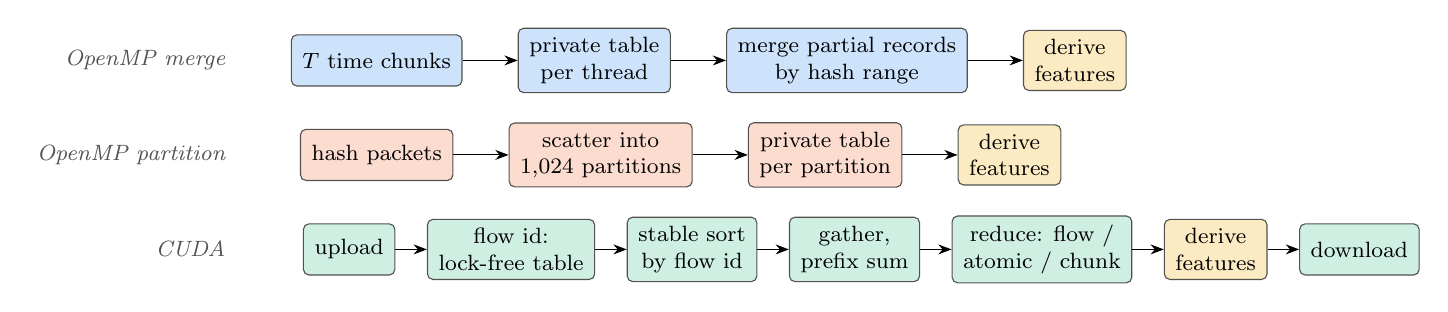
\begin{tikzpicture}[font=\footnotesize, >=Stealth,
  box/.style={draw=ink2, rounded corners=2pt, minimum height=6.5mm, inner xsep=4pt, align=center},
  lab/.style={font=\footnotesize\itshape, text=ink2, anchor=east}]
% row 1: merge
\node[lab] at (-0.2,2.4) {OpenMP merge};
\node[box, fill=b1] (m1) at (1.6,2.4) {$T$ time chunks};
\node[box, fill=b1, right=7mm of m1] (m2) {private table\\per thread};
\node[box, fill=b1, right=7mm of m2] (m3) {merge partial records\\by hash range};
\node[box, fill=y1, right=7mm of m3] (m4) {derive\\features};
\draw[->] (m1)--(m2); \draw[->] (m2)--(m3); \draw[->] (m3)--(m4);
% row 2: partition
\node[lab] at (-0.2,1.2) {OpenMP partition};
\node[box, fill=o1] (p1) at (1.6,1.2) {hash packets};
\node[box, fill=o1, right=7mm of p1] (p2) {scatter into\\1{,}024 partitions};
\node[box, fill=o1, right=7mm of p2] (p3) {private table\\per partition};
\node[box, fill=y1, right=7mm of p3] (p4) {derive\\features};
\draw[->] (p1)--(p2); \draw[->] (p2)--(p3); \draw[->] (p3)--(p4);
% row 3: GPU
\node[lab] at (-0.2,0) {CUDA};
\node[box, fill=g1] (g0) at (1.25,0) {upload};
\node[box, fill=g1, right=4mm of g0] (g1) {flow id:\\lock-free table};
\node[box, fill=g1, right=4mm of g1] (g2) {stable sort\\by flow id};
\node[box, fill=g1, right=4mm of g2] (g3) {gather,\\prefix sum};
\node[box, fill=g1, right=4mm of g3] (g4) {reduce: flow /\\atomic / chunk};
\node[box, fill=y1, right=4mm of g4] (g5) {derive\\features};
\node[box, fill=g1, right=4mm of g5] (g6) {download};
\draw[->] (g0)--(g1); \draw[->] (g1)--(g2); \draw[->] (g2)--(g3); \draw[->] (g3)--(g4); \draw[->] (g4)--(g5); \draw[->] (g5)--(g6);
\end{tikzpicture}
\caption{The three parallel pipelines. Every row starts from the same
time-ordered packet batch and ends with the same flow records.}
\label{fig:pipeline}
\end{figure*}

\subsection{CUDA pipeline}
The GPU version (Fig.~\ref{fig:pipeline}) does not update a table packet by
packet. It regroups the packets so that every feature becomes a reduction over
a contiguous segment.

\emph{1. Flow identifier.} One thread per packet inserts the key in a
lock-free open-addressing table~\cite{alcantara}. A slot is a single 32-bit
word that stores the index of the packet that claimed it, so one
compare-and-swap inserts a 13-byte key, and keys are compared through that
packet. The slot index identifies the flow exactly; no hash collisions are
tolerated.

\emph{2. Sort.} A stable radix sort from Thrust~\cite{thrust} orders the packet
indices by flow identifier. The packets of a flow become contiguous and remain
in time order.

\emph{3. Gather.} Timestamps and lengths are copied into sorted order, so the
following kernels read memory sequentially (coalesced access). A prefix sum
over the flow boundaries numbers the flows.

\emph{4. Reduce.} After sorting, the inter-arrival time of a packet is the
difference with its left neighbor, so every feature is a sum, minimum or
maximum over a segment. We implemented three kernels. \code{gpu-flow} uses one
thread per flow, which walks the packets of its flow. \code{gpu-atomic} uses
one thread per packet, which adds its contribution to the record of its flow
with atomic instructions. \code{gpu-chunk} uses one thread per chunk of $c$
consecutive sorted packets; it accumulates in registers while the flow does
not change and issues one atomic update per flow met in the chunk. Burst
lengths are obtained by compacting the positions where bursts start.

\emph{5. Derive and download.} A kernel derives the statistical features, and
records are copied back to the host.

\subsection{MPI4Py distribution}
Captures are processed as independent batches, which fits distributed
memory: a driver written with MPI4Py gives batches to processes, and each
process calls the C++ kernel through a shared library. With the \emph{static}
schedule, each process takes a contiguous block of the batch list. With the
\emph{dynamic} schedule, every process takes the next unclaimed batch from a
shared counter that is advanced with a one-sided fetch-and-add operation,
largest batches first. Process 0 collects either a summary per batch or all
the flow records (\code{Gatherv}).

\subsection{Correctness and quality metric}
The application-specific quality metric is \emph{flow-record accuracy}: the
fraction of flows whose record is identical to the reference. The reference
chain has two links. First, the sequential baseline is compared with an
independent implementation written in plain Python, which groups packets in
a dictionary and computes every feature from the full packet list of the
flow. Second, every parallel version is compared with the baseline: integer
accumulators must be identical and derived features must agree within a
relative tolerance of $10^{-9}$. The test suite covers edge cases (one
packet, one flow, all flows distinct, more threads than packets, odd thread
counts, extreme burst gaps), all GPU launch configurations, the MPI driver and
the real trace. During the benchmarks, every run also reports a checksum of
its records, and the driver stops if two versions disagree on the same input.

\subsection{Code and data availability}
The source code, build instructions, configuration files, raw results and the
scripts that regenerate every figure and table are in the open repository
\url{https://github.com/Bunnydragon96/hpc-flow-feature-extraction}. The
synthetic data are generated by the programs. The real trace is downloaded
from the MAWI archive~\cite{mawi} with the command given in the repository.

\section{Results}

\subsection{Experimental setting}
The main platform is a Linux virtual machine with 8 virtual processors of an
Intel Core i7-6700 (3.4\,GHz, a processor with 4 cores and 8 hardware threads),
19\,GiB of memory and an NVIDIA Quadro P2000 GPU (5\,GiB, 2017). The software is
Ubuntu 24.04, the GNU Compiler Collection (GCC) 13.3 with \code{-O3 -march=native}, CUDA 12.0, Open MPI 4.1.6
and MPI4Py 4.1.2. A second platform, used for the processor versions only, is
an Apple M4 with 4 performance and 6 efficiency cores and GCC 16.2.

Each configuration runs 2 warm-up repetitions and 7 timed repetitions in one
process, and we report the median. The time covers everything from packets in
host memory to flow records in host memory; for the GPU it includes the upload
and the download. Reading or generating the input is excluded. Large buffers
are recycled between repetitions, as a pipeline that processes one batch after
another would do. Speedup is $S = T_{\mathrm{seq}}/T_{\mathrm{par}}$, measured
against the sequential baseline on the same input, and efficiency is $E = S/p$
for $p$ threads or processes. Unless stated otherwise, synthetic inputs have
$2^{24}$ packets and $2^{20}$ flows.

\subsection{Correctness}
All \nchecks{} checks of the test suite pass on the main platform and all
\nchecksMac{} on the second one. Flow-record accuracy is 100\%: the integer
accumulators of every parallel version are identical to the baseline, and the
largest relative difference in a derived feature is below $10^{-15}$ (the
entropy, which uses a logarithm). The baseline agrees with the independent
Python reference on all its inputs, including the first 60{,}000 packets of the
real trace.

\subsection{Runtime and speedup versus problem size}
Fig.~\ref{fig:size} shows the throughput for $2^{20}$ to $2^{25}$ packets with
moderate skew ($s=1$, $n/16$ flows). At $2^{25}$ packets the baseline needs
3.24\,s (\sizeSeqMpps{} million packets per second). The speedups are
\sizeChunkSp\x{} for \code{gpu-chunk}, \sizePartSp\x{} for \code{omp-part},
\sizeAtomicSp\x{} for \code{gpu-atomic}, \sizeFlowSp\x{} for \code{gpu-flow} and
\sizeMergeSp\x{} for \code{omp-merge}. The baseline slows down as the batch
grows, from \sizeSeqSmallMpps{} to \sizeSeqMpps{} million packets per second,
because its table stops fitting in the cache. The partitioned and GPU
versions keep an almost constant throughput, so their speedup grows with the
problem size.

\begin{figure}[H]
\centering
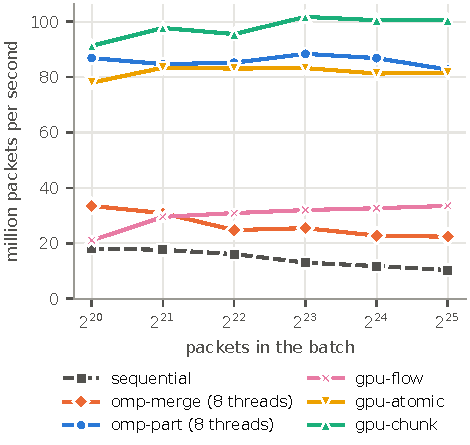
\includegraphics[width=\linewidth]{throughput_vs_size.pdf}
\caption{Throughput versus batch size on synthetic traffic ($s=1$). OpenMP
versions use 8 threads. Higher is better.}
\label{fig:size}
\end{figure}

\subsection{Effect of skew and of the number of flows}
Table~\ref{tab:skew} and Fig.~\ref{fig:skew} vary the Zipf exponent. Three
effects appear.

First, skew helps the baseline: it is \skewSeqRatio\x{} faster at $s=2$ than at
$s=0$, because the popular records stay in the cache. Table~\ref{tab:flows}
isolates this effect with uniform traffic: the baseline costs
\flowsSeqNsSmall\,ns per packet with 256 flows and \flowsSeqNsBig\,ns with 4
million flows.

Second, the two OpenMP strategies react in opposite ways. \code{omp-part} is
\skewPartSpZero\x{} faster than the baseline at $s=0$ but only
\skewPartSpTwo\x{} at $s=2$: the largest flow has \topshareTwo\% of the packets
and its partition is processed by one thread. \code{omp-merge} is weak with
many flows (\skewMergeSpZero\x{} at $s=0$), because every thread builds a table
almost as large as the global one and the merge repeats the work, and it is
the best processor version under heavy skew (\skewMergeSpHi\x{} at $s=1.5$).

Third, on the GPU the kernel with one thread per flow is the fastest for
uniform traffic and collapses with skew: at $s=2$ it is \skewFlowSlow\x{}
slower than \code{gpu-chunk} and 12 times slower than the baseline, because
one GPU thread walks 10 million packets. \code{gpu-atomic} is stable, and
\code{gpu-chunk} is the best or close to the best for every $s \ge 0.8$.

\begin{table}[H]
\centering\footnotesize
\setlength{\tabcolsep}{3.2pt}
\caption{Runtime in milliseconds versus Zipf exponent $s$ ($2^{24}$ packets).
The best time of each column is in bold.}\label{tab:skew}
\begin{tabular}{@{}l rrrrrrr@{}}
\toprule
$s$ & 0 & 0.5 & 0.8 & 1.0 & 1.2 & 1.5 & 2.0 \\
\midrule
\tabinput{tables/skew_short.tex}
\bottomrule
\end{tabular}
\end{table}

\begin{figure}[H]
\centering
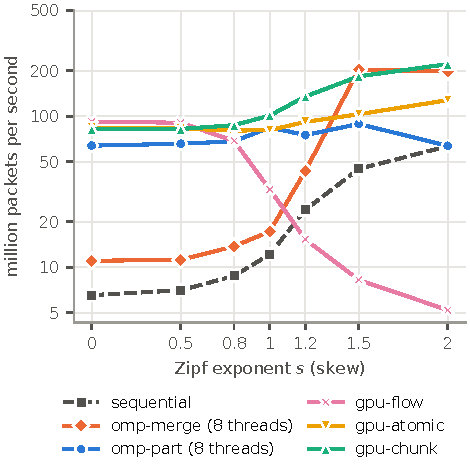
\includegraphics[width=\linewidth]{throughput_vs_skew.pdf}
\caption{Throughput versus skew (logarithmic vertical axis), same runs as
Table~\ref{tab:skew}.}
\label{fig:skew}
\end{figure}

\begin{table}[H]
\centering\footnotesize
\setlength{\tabcolsep}{4pt}
\caption{Runtime in milliseconds versus number of flows (uniform traffic,
$2^{24}$ packets). Best time per column in bold.}\label{tab:flows}
\begin{tabular}{@{}l rrrrrr@{}}
\toprule
Flows & $2^{8}$ & $2^{12}$ & $2^{16}$ & $2^{18}$ & $2^{20}$ & $2^{22}$ \\
\midrule
\tabinput{tables/flows.tex}
\bottomrule
\end{tabular}
\end{table}

\subsection{Strong and weak scaling with OpenMP}
Fig.~\ref{fig:scaling}(a,b) and Table~\ref{tab:strong} show strong scaling.
For \code{omp-part} at $s=0$ the speedup over the baseline is
\ssPartZeroFour\x{} with 4 threads, an efficiency above 100\%. This is not only
parallelism: with one thread the partitioned algorithm is already
\ssPartZeroOne\x{} faster than the baseline because each partition fits in the
cache. Against its own one-thread time, 4 threads give \ssPartZeroSelfFour\x{}
and 8 threads \ssPartZeroSelf\x. The curves flatten after 4 threads
because the machine has 4 physical cores. At $s=1.5$ the load imbalance limits
\code{omp-part} to \ssPartHiEight\x, while \code{omp-merge} reaches
\ssMergeHiEight\x{} (\ssMergeHiSelf\x{} against its own one-thread time).

\begin{figure*}[t]
\centering
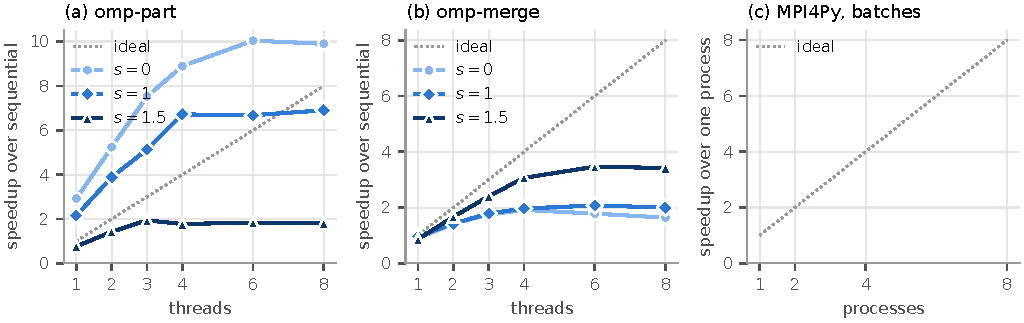
\includegraphics[width=\linewidth]{scaling.pdf}
\caption{Strong scaling. (a), (b): speedup of the two OpenMP strategies over
the sequential baseline for three skews ($2^{24}$ packets). (c): speedup of the
MPI4Py driver over one process, for 30 real batches and for 16 synthetic
batches of uneven size, with static and dynamic schedules. The dotted line is
the ideal speedup.}
\label{fig:scaling}
\end{figure*}

\begin{table}[H]
\centering\footnotesize
\setlength{\tabcolsep}{3.4pt}
\caption{Strong scaling on the main platform. $T_{\mathrm{seq}}$ in
milliseconds; speedup over the baseline with 1 to 8 threads; $E_8$ is the
efficiency with 8 threads; ``self'' is the speedup of 8 threads over 1 thread
of the same strategy.}\label{tab:strong}
\begin{tabular}{@{}l r r rrrr r r@{}}
\toprule
 & $s$ & $T_{\mathrm{seq}}$ & 1 & 2 & 4 & 8 & $E_8$ & self \\
\midrule
\tabinput{tables/strong.tex}
\bottomrule
\end{tabular}
\end{table}

For weak scaling (Table~\ref{tab:weak}) the input grows with the thread
count, $2^{22}$ packets and $2^{18}$ flows per thread. Efficiency falls to
\weakPartEff\% for \code{omp-part} and \weakMergeEff\% for \code{omp-merge} at
8 threads. Two causes add up: only 4 cores are available, and the cost per
packet itself grows with the number of flows (the baseline takes 11 times
longer for 8 times more data).

\begin{table}[H]
\centering\footnotesize
\setlength{\tabcolsep}{3.6pt}
\caption{Weak scaling ($s=1$): runtime in milliseconds and efficiency
$T(1)/T(p)$ of each strategy.}\label{tab:weak}
\begin{tabular}{@{}r r r rr rr@{}}
\toprule
 & & & \multicolumn{2}{c}{omp-part} & \multicolumn{2}{c}{omp-merge} \\
Threads & Packets & seq & time & eff. & time & eff. \\
\midrule
\tabinput{tables/weak.tex}
\bottomrule
\end{tabular}
\end{table}

Table~\ref{tab:mac} repeats the experiment on the Apple M4, including the
one-minute real batch. The pattern is the same, and the programs scale
further: \code{omp-part} reaches \macPartZeroTen\x{} over the baseline with 10
threads at $s=0$, and \code{omp-merge} reaches \macMergeHiTen\x{} at $s=1.5$.
Gains are smaller beyond 4 threads, where the efficiency cores come into use.

\begin{table}[H]
\centering\footnotesize
\setlength{\tabcolsep}{3pt}
\caption{Second platform (Apple M4): $T_{\mathrm{seq}}$ in milliseconds and
speedup over the baseline with 1 to 10 threads, for synthetic traffic and for
the one-minute real batch.}\label{tab:mac}
\begin{tabular}{@{}l r r rrrrrr@{}}
\toprule
 & $s$ & $T_{\mathrm{seq}}$ & 1 & 2 & 4 & 6 & 8 & 10 \\
\midrule
\tabinput{tables/mac.tex}
\bottomrule
\end{tabular}
\end{table}

\subsection{Contention on a shared table}\label{sec:contention}
Fig.~\ref{fig:contention} shows the micro-benchmark that motivates avoiding a
shared table. It computes only the order-independent features. With uniform
traffic, 8 threads on a shared table are \contLockZero\x{} (locks) and
\contAtomicZero\x{} (atomics) faster than one thread. At $s=1.5$ the shared
table with locks drops to \contLockHiMpps{} million packets per second, 3 times
\emph{slower} than one thread (\contSeqHi{} million), and at $s=2$ it is
\contLockTwo{} times slower: the threads take turns on the record of the
largest flow and its cache line moves between cores on every update. Private
tables with a merge reach \contLocalHiMpps{} million packets per second at
$s=1.5$.

\begin{figure}[H]
\centering
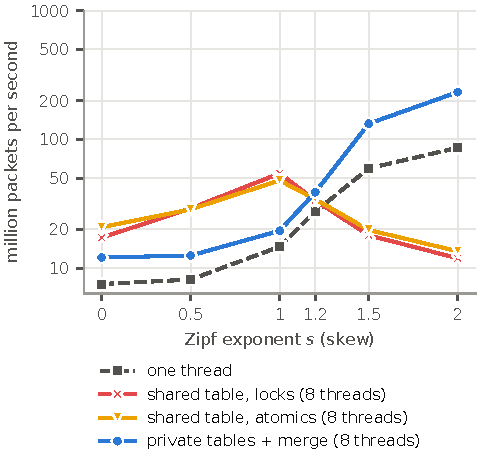
\includegraphics[width=\linewidth]{contention.pdf}
\caption{Shared hash table under skew: throughput of the order-independent
aggregation ($2^{24}$ packets, $2^{18}$ flows, logarithmic axis).}
\label{fig:contention}
\end{figure}

\subsection{GPU: time breakdown, transfers and launch configuration}
Fig.~\ref{fig:gpu} splits the time of \code{gpu-chunk}. For synthetic traffic
at $s=1$, grouping takes \gpuOneGroupShare\% and the two transfers
\gpuOneXferShare\%. For the real trace the download alone takes
\gpuRealDownShare\%: the batch is \xferRealInMB\,MB of packets but produces
\xferRealOutMB\,MB of records, because it has 3.2 million flows of 248 bytes
each.

\begin{figure}[H]
\centering
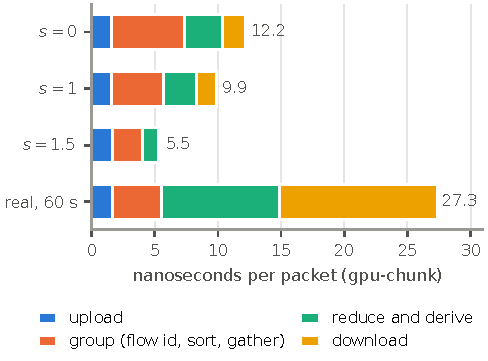
\includegraphics[width=\linewidth]{gpu_breakdown.pdf}
\caption{Time of \code{gpu-chunk} per packet, by stage. The number at the end
of each bar is the total in nanoseconds per packet.}
\label{fig:gpu}
\end{figure}

\emph{Memory transfers.} Uploading from page-locked host memory reaches
\xferUpPinDirect\,GB/s against \xferUpPageDirect\,GB/s from pageable memory.
For the download, copying directly into the recycled result buffer
(\xferDownPinDirect\,GB/s) is faster than downloading into page-locked memory
and copying again (\xferDownPinStaged\,GB/s). The best combination processes
the real batch in \xferTotalPinDirect\,ms and the worst in
\xferTotalPageStaged\,ms.

\emph{Launch configuration.} Table~\ref{tab:gpucfg} shows that the number of
threads per block matters little: the kernels are simple maps limited by
memory, and the spread is \tpbSpreadAtomic\% for \code{gpu-atomic} and
\tpbSpreadChunk\% for \code{gpu-chunk}. The chunk size matters a lot. With one
packet per thread and $s=1.5$ the reduction takes \chunkHiOne\,ms, because
thousands of threads update the same record atomically. With 8 packets per
thread it takes \chunkHiBest\,ms. Larger chunks are slower again
(\chunkHiLast\,ms at 255) because each thread then reads a long private range
and neighboring threads no longer touch neighboring memory. We use 8 as the
default.

\begin{table}[H]
\centering\footnotesize
\setlength{\tabcolsep}{2.6pt}
\caption{GPU launch configuration, times in milliseconds, best per row in
bold. Top: total time versus threads per block ($s=1$). Bottom: time of the
reduction stage of \code{gpu-chunk} versus packets per thread.}\label{tab:gpucfg}
\begin{tabular}{@{}l rrrrrr@{}}
\toprule
Threads per block & 32 & 64 & 128 & 256 & 512 & 1024 \\
\midrule
\tabinput{tables/gpu_tpb.tex}
\bottomrule
\end{tabular}

\vspace{4pt}
\begin{tabular}{@{}l rrrrrrrrr@{}}
\toprule
Chunk & 1 & 2 & 4 & 8 & 16 & 32 & 64 & 128 & 255 \\
\midrule
\tabinput{tables/gpu_chunk.tex}
\bottomrule
\end{tabular}
\end{table}

\subsection{Real backbone traffic}
Table~\ref{tab:real} gives the results on the real trace. In one minute,
\realSingle\% of the flows have a single packet, and \realHalfFlows{} flows
(\realHalfPct\% of them) carry half of the packets. The three GPU kernels are
equivalent here, about 4.3\x{} faster than the baseline (\realChunkMpps{}
million packets per second), and the speedup holds up to the largest batch
that fits in the 5\,GiB of the GPU. \code{omp-part} reaches \realPartSp\x{} and
\code{omp-merge} \realMergeSp\x. The gains are smaller than on synthetic
traffic because there is one record for every 2.4 packets: producing 789\,MB
of output is a large part of the work for every version.

On the Apple M4 (Table~\ref{tab:mac}) the baseline processes the one-minute
batch in \macRealSeq\,ms (\macRealSeqMpps{} million packets per second) and
\code{omp-part} is \macRealPartBest\x{} faster with 8 threads. That is
81\,ms, less than the \xferTotalPinDirect\,ms of the GPU pipeline on the
main platform: a current processor with the partitioned algorithm outruns
this 2017 GPU on mice-dominated traffic.

\begin{table}[H]
\centering\footnotesize
\setlength{\tabcolsep}{3.4pt}
\caption{Real trace: runtime in milliseconds and speedup over the baseline
for batches of 60, 120 and 240 seconds. OpenMP versions use 8 threads. Best
speedup per batch in bold.}\label{tab:real}
\begin{tabular}{@{}l rr rr rr@{}}
\toprule
 & \multicolumn{2}{c}{60 s} & \multicolumn{2}{c}{120 s} & \multicolumn{2}{c}{240 s} \\
 & ms & $S$ & ms & $S$ & ms & $S$ \\
\midrule
\tabinput{tables/real.tex}
\bottomrule
\end{tabular}
\end{table}

\subsection{Distributed batches with MPI4Py}
The 15-minute trace was cut into 30 batches of 30 seconds
(\mpiPackets{} million packets, \mpiFlows{} million flow records in total).
Table~\ref{tab:mpi} and Fig.~\ref{fig:scaling}(c) show the results with the
sequential kernel in every process. One process needs \mpiOneWall\,s. With 4
processes the speedup is \mpiStaticSpFour\x, and with 8 it is only
\mpiStaticSp\x{} (efficiency \mpiStaticEff\%). The cause is not communication:
the summaries are tiny and the shared counter of the dynamic schedule costs
\mpiSchedMs\,ms in total. The kernel is limited by memory. When we run
independent copies of the sequential program on one batch, each copy takes
0.50\,s alone, 0.81\,s with 4 copies and 1.53\,s with 8 copies. The same test
on an input that fits in the cache takes 0.23\,s alone, 0.24\,s with 4 copies
and 0.56\,s with 8, which is the effect of having 4 physical cores.

\begin{table}[H]
\centering\footnotesize
\setlength{\tabcolsep}{3pt}
\caption{MPI4Py strong scaling: wall time in seconds and speedup $S$ over one
process, for the real batches and for the batches of uneven size.}\label{tab:mpi}
\begin{tabular}{@{}r rr rr rr rr@{}}
\toprule
 & \multicolumn{4}{c}{30 real batches} & \multicolumn{4}{c}{16 uneven batches} \\
 & \multicolumn{2}{c}{static} & \multicolumn{2}{c}{dynamic} & \multicolumn{2}{c}{static} & \multicolumn{2}{c}{dynamic} \\
$p$ & s & $S$ & s & $S$ & s & $S$ & s & $S$ \\
\midrule
\tabinput{tables/mpi.tex}
\bottomrule
\end{tabular}
\end{table}

\emph{Load balance.} The real batches have similar sizes, so static and
dynamic schedules perform the same. The uneven set has two batches of
$2^{24}$ packets followed by fourteen of $2^{21}$. With 4 processes the static
schedule gives both large batches to process 0 and reaches
\mpiUnevenStaticSpFour\x, while the dynamic schedule reaches
\mpiUnevenDynSpFour\x. With 8 processes on 4 cores both become slower than
with 4.

\emph{Other measurements.} In weak scaling (3 real batches per process) the
efficiency is \mpiWeakEff\% at 8 processes, for the same memory reason.
Collecting all flow records at process 0 instead of summaries is expensive:
for 8 batches (\mpiCollectGB\,GB of records) and 8 processes the wall time
grows \mpiCollectSlow\x{} and the collection takes \mpiCollectShare\% of it. A
real deployment should write the records where they are produced. Finally,
combining both models, 2 processes with 4 threads of \code{omp-part} each
process the whole trace in \mpiHybridBestS\,s (\mpiHybridBestMpps{} million
packets per second), \mpiHybridSp\x{} faster than one sequential process.

\section{Conclusions}
We built a packet-to-flow feature extraction pipeline with a sequential
baseline, two OpenMP strategies, a CUDA pipeline with three reduction kernels
and an MPI4Py driver, and verified that all of them produce identical flow
records. On synthetic traffic the GPU version is up to \sizeChunkSp\x{} faster
than the baseline and 8 threads up to \skewPartSpZero\x; on a real backbone
trace the gains are 4.3\x{} and \realPartSp\x.

The main lesson is that grouping performance depends on the shape of the
traffic more than on the programming model. Many flows make the problem
memory-bound; partitioning by flow hash then helps even with one thread. A
dominant flow breaks every scheme that gives a flow to a single worker
(a partition, a GPU thread) and makes a shared table slower than one thread;
schemes that split the packets evenly and combine partial results (the merge
on the processor, the chunked kernel on the GPU) are robust to it. Real traffic
shows both problems at once, and its many single-packet flows make the output
transfer the largest GPU cost. Parallel resources beyond the 4 physical cores
of the test machine gave no benefit, for threads and for processes alike.

Future work: choose the strategy at run time from a sample of the batch; run
the MPI driver on several nodes, where memory is not shared; process
captures larger than GPU memory in pieces using the merge operation; and add
bidirectional flows and flow timeouts as flow exporters use.

\section*{References}
\begingroup
\footnotesize
\renewcommand{\section}[2]{}
\begin{thebibliography}{99}
\setlength{\itemsep}{1pt}
\bibitem{netflow} B. Claise. Cisco Systems NetFlow services export version 9. \emph{Request for Comments 3954, Internet Engineering Task Force}, 2004.
\bibitem{cicflowmeter} A. H. Lashkari, G. Draper-Gil, M. S. I. Mamun, and A. A. Ghorbani. Characterization of Tor traffic using time based features. \emph{International Conference on Information Systems Security and Privacy}, pages 253--262, 2017.
\bibitem{cicids} I. Sharafaldin, A. H. Lashkari, and A. A. Ghorbani. Toward generating a new intrusion detection dataset and intrusion traffic characterization. \emph{International Conference on Information Systems Security and Privacy}, pages 108--116, 2018.
\bibitem{elephants} C. Estan and G. Varghese. New directions in traffic measurement and accounting. \emph{ACM SIGCOMM}, pages 323--336, 2002.
\bibitem{cieslewicz} J. Cieslewicz and K. A. Ross. Adaptive aggregation on chip multiprocessors. \emph{International Conference on Very Large Data Bases}, pages 339--350, 2007.
\bibitem{balkesen} C. Balkesen, J. Teubner, G. Alonso, and M. T. \"Ozsu. Main-memory hash joins on multi-core CPUs: tuning to the underlying hardware. \emph{IEEE International Conference on Data Engineering}, pages 362--373, 2013.
\bibitem{alcantara} D. A. Alcantara, A. Sharf, F. Abbasinejad, S. Sengupta, M. Mitzenmacher, J. D. Owens, and N. Amenta. Real-time parallel hashing on the GPU. \emph{ACM Transactions on Graphics}, 28(5), pages 1--9, 2009.
\bibitem{thrust} N. Bell and J. Hoberock. Thrust: a productivity-oriented library for CUDA. \emph{GPU Computing Gems Jade Edition}, pages 359--371, 2012.
\bibitem{openmp} L. Dagum and R. Menon. OpenMP: an industry standard API for shared-memory programming. \emph{IEEE Computational Science and Engineering}, 5(1), pages 46--55, 1998.
\bibitem{cuda} J. Nickolls, I. Buck, M. Garland, and K. Skadron. Scalable parallel programming with CUDA. \emph{ACM Queue}, 6(2), pages 40--53, 2008.
\bibitem{mpi4py} L. Dalc\'in, R. Paz, and M. Storti. MPI for Python. \emph{Journal of Parallel and Distributed Computing}, 65(9), pages 1108--1115, 2005.
\bibitem{mawi} K. Cho, K. Mitsuya, and A. Kato. Traffic data repository at the WIDE project. \emph{USENIX Annual Technical Conference, FREENIX Track}, pages 263--270, 2000.
\end{thebibliography}
\endgroup


\end{document}
